% P3 Feature Engineering, Weather Integration & Ablation Contributions (Phase B)
% Sections intended for inclusion in reports/report.tex

\subsection{Prediction Checkpoints and Full-Scale Feature Architecture}
The departure delay prediction task is framed as a binary classification problem: predicting whether a scheduled commercial domestic flight will depart its origin gate with a delay $\ge 15$ minutes ($\text{LATE} = 1$) or $< 15$ minutes ($\text{LATE} = 0$), based on reconstructed UTC gate departure timestamps ($\text{OBSERVED} - \text{TIME}$).

Features are computed strictly relative to two pre-departure prediction checkpoints:
\begin{enumerate}
    \item \textbf{Strategic Dispatch Horizon ($T = 360\text{ min}$ / $6\text{h}$):} Models early-day dispatch planning and baseline weather regimes before surface queues build.
    \item \textbf{Tactical Gate Horizon ($T = 60\text{ min}$ / $1\text{h}$):} Models gate operations, recent surface weather observations, 3-hour origin departure congestion, and inbound aircraft arrival status.
\end{enumerate}

All full-scale Phase B feature matrices cover the complete $5{,}749{,}041$-row arrival-audited development cohort (\texttt{flights\_development\_phase\_b.parquet}), using all development records as historical context while preserving strict positional index invariance ($\text{index}(X) \equiv \text{index}(\text{df})$).

\subsection{Anti-Leakage Safeguards and Weather Integration}
The feature pipeline (\texttt{src/features.py} and \texttt{src/weather.py}) enforces four protocol guarantees:
\begin{itemize}
    \item \textbf{Strict Cutoff Rule:} No event timestamped after $\text{cutoff}_T = \text{TIME} - \Delta T$ enters computation.
    \item \textbf{Target Self-Exclusion:} Origin airport 3-hour congestion (\texttt{origin\_departures\_3h}, \texttt{origin\_late\_rate\_3h}) excludes the target flight itself when present in the history pool, even if it pushed back early. Cancellation rates are excluded because BTS records do not timestamp when cancellations were announced.
    \item \textbf{Hourly Surface Weather Join (Decision D2):} Routine METAR and SPECI observations ($3{,}826{,}099$ records covering $347/349$ origin airports, Jan 2025--Jan 2026) were retrieved from the public-domain Iowa Environmental Mesonet (IEM) ASOS archive and joined via strict backward \texttt{merge\_asof} ($\text{obs\_time\_utc} \le \text{cutoff}_T$). Observations older than $6\text{h}$ or from unmapped stations trigger \texttt{weather\_missing} $= 1$ without silent imputation.
    \item \textbf{Decision D1 Quarantine (Tail-Chain Features):} Because BTS reports retrospective final tail numbers rather than live dispatch assignments, inbound aircraft features are omitted from the proposed primary set (\textbf{G2}) and isolated in \textbf{G3} as an ablation under the operational-feed assumption.
\end{itemize}

\subsection{Feature-Group Ablation Analysis}
To quantify how much predictive signal each information source contributes across horizons, we evaluated four nested feature groups (\textbf{G0}: schedule/route; \textbf{G1}: $+$ 3h origin congestion; \textbf{G2}: $+$ origin surface weather; \textbf{G3}: $+$ inbound tail chain) using a fixed LightGBM pipeline at feature-code revision \texttt{c9f5560494b52d370448e57264ec2109e74a6909} across all 4 rolling validation folds and 3 seeds ($42, 73, 101$). Spreads are reported as population standard deviation ($\text{ddof}=0$) matching the project evaluation harness.

\begin{table}[h]
\centering
\caption{Phase B feature-group ablation on the 5.75M development cohort (LightGBM, revision \texttt{c9f5560}, mean $\pm$ population std ($\text{ddof}=0$) across 4 folds $\times$ 3 seeds).}
\label{tab:p3-ablation}
\begin{tabular}{llcc}
\hline
\textbf{Group} & \textbf{Checkpoint} & \textbf{Val PR-AUC} & \textbf{Val ROC-AUC} \\
\hline
G0: Schedule \& Route & 360 min (6h) & $0.366 \pm 0.067$ & $0.688 \pm 0.010$ \\
G0: Schedule \& Route & 60 min (1h)  & $0.366 \pm 0.067$ & $0.688 \pm 0.010$ \\
G1: $+$ Origin Congestion (3h) & 360 min (6h) & $0.381 \pm 0.069$ & $0.693 \pm 0.010$ \\
G1: $+$ Origin Congestion (3h) & 60 min (1h)  & $0.415 \pm 0.066$ & $0.705 \pm 0.009$ \\
G2: $+$ Surface Weather (D2) & 360 min (6h) & $0.381 \pm 0.070$ & $0.693 \pm 0.011$ \\
G2: $+$ Surface Weather (D2) & 60 min (1h)  & $0.417 \pm 0.067$ & $0.706 \pm 0.010$ \\
G3: $+$ Tail Chain (D1 ablation) & 360 min (6h) & $0.381 \pm 0.069$ & $0.695 \pm 0.011$ \\
G3: $+$ Tail Chain (D1 ablation) & 60 min (1h)  & $0.542 \pm 0.060$ & $0.793 \pm 0.006$ \\
\hline
\end{tabular}
\end{table}

At $T = 6\text{h}$, origin congestion provides a modest $+0.014$ PR-AUC gain over schedule alone, while weather and inbound rotation add negligible signal ($< 0.001$). At $T = 1\text{h}$, recent origin congestion adds $+0.049$ PR-AUC ($0.366 \to 0.415$) and surface weather adds $+0.002$ PR-AUC ($0.415 \to 0.417$). Under the Decision D1 operational-feed assumption (\textbf{G3}), inbound aircraft continuity yields a $+0.125$ PR-AUC jump ($0.417 \to 0.542$, ROC-AUC $0.793$), showing the largest measured increase among the groups under the retrospective assignment assumption. Figure~\ref{fig:p3-ablation} visualizes this progression across horizons.

\begin{figure}[h]
\centering
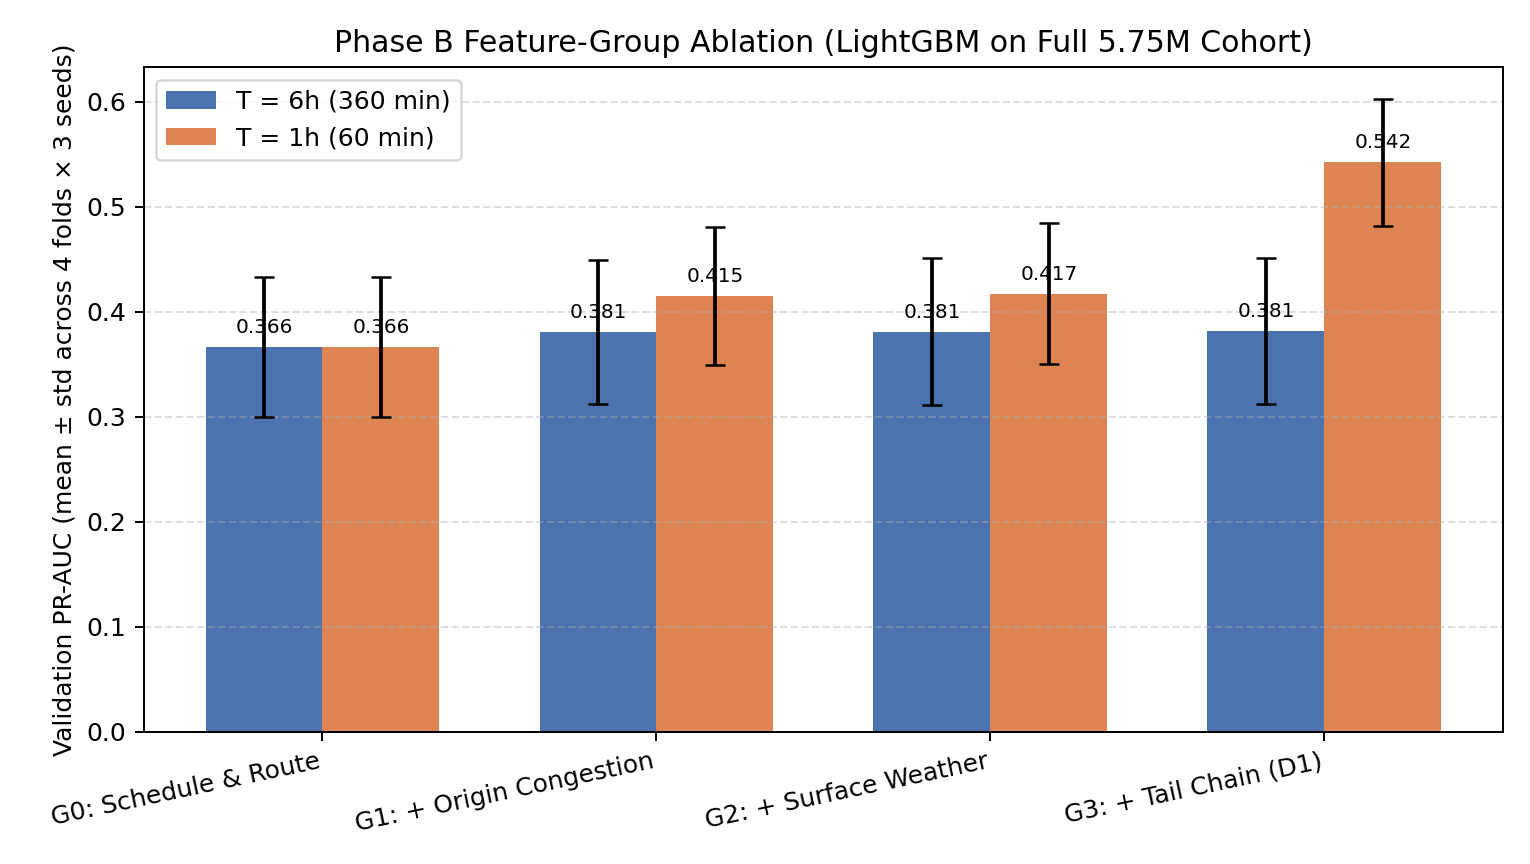
\includegraphics[width=0.88\linewidth]{figures/p3_ablation_chart.png}
\caption{Validation PR-AUC across feature groups G0--G3 at the 6h and 1h checkpoints.}
\label{fig:p3-ablation}
\end{figure}
